\documentclass[border=10pt]{standalone}
\usepackage{pgfplots}
\pgfplotsset{compat=1.18}
\begin{document}
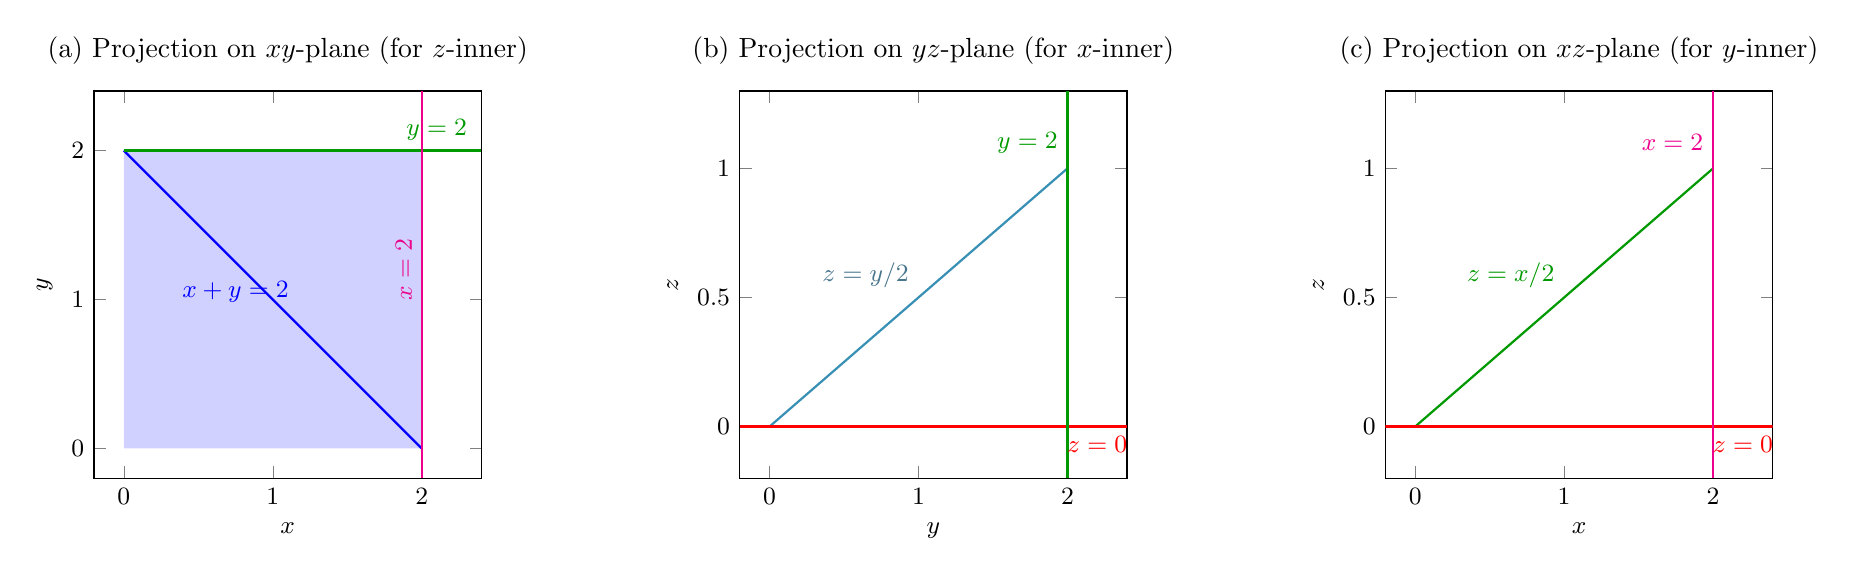
\begin{tikzpicture}
% (a) xy-plane projection
\begin{axis}[
    at={(0cm,0cm)}, anchor=west,
    width=6.5cm, height=6.5cm,
    xmin=-0.2, xmax=2.4, ymin=-0.2, ymax=2.4,
    xlabel={$x$}, ylabel={$y$},
    title={(a) Projection on $xy$-plane (for $z$-inner)},
    tick label style={font=\small}, label style={font=\small},
]
\addplot[fill=blue!30, opacity=0.6, draw=none] coordinates {(0,2) (2,2) (2,0)} \closedcycle;
\addplot[blue, thick, domain=0:2] {2-x};
\addplot[green!60!black, thick] coordinates {(0,2) (2.4,2)};
\addplot[magenta, thick] coordinates {(2,-0.2) (2,2.4)};
\node[blue, font=\small] at (axis cs:0.75,1.05) {$x+y=2$};
\node[green!60!black, font=\small, above] at (axis cs:2.1,2) {$y=2$};
\node[magenta, font=\small, rotate=90, anchor=south] at (axis cs:2,1.2) {$x=2$};
\end{axis}
% (b) yz-plane projection
\begin{axis}[
    at={(8.2cm,0cm)}, anchor=west,
    width=6.5cm, height=6.5cm,
    xmin=-0.2, xmax=2.4, ymin=-0.2, ymax=1.3,
    xlabel={$y$}, ylabel={$z$},
    title={(b) Projection on $yz$-plane (for $x$-inner)},
    tick label style={font=\small}, label style={font=\small},
]
\addplot[fill=cyan!40, opacity=0.6, draw=none] coordinates {(0,0) (2,0) (2,1)} \closedcycle;
\addplot[cyan!70!black, thick, domain=0:2] {x/2};
\addplot[red, thick] coordinates {(-0.2,0) (2.4,0)};
\addplot[green!60!black, thick] coordinates {(2,-0.2) (2,1.3)};
\node[cyan!50!black, font=\small, above left] at (axis cs:1,0.5) {$z=y/2$};
\node[red, font=\small, below] at (axis cs:2.2,0) {$z=0$};
\node[green!60!black, font=\small, left] at (axis cs:2,1.1) {$y=2$};
\end{axis}
% (c) xz-plane projection
\begin{axis}[
    at={(16.4cm,0cm)}, anchor=west,
    width=6.5cm, height=6.5cm, 
    xmin=-0.2, xmax=2.4, ymin=-0.2, ymax=1.3,
    xlabel={$x$}, ylabel={$z$},
    title={(c) Projection on $xz$-plane (for $y$-inner)},
    tick label style={font=\small}, label style={font=\small},
]
\addplot[fill=green!40, opacity=0.6, draw=none] coordinates {(0,0) (2,0) (2,1)} \closedcycle;
\addplot[green!60!black, thick, domain=0:2] {x/2};
\addplot[red, thick] coordinates {(-0.2,0) (2.4,0)};
\addplot[magenta, thick] coordinates {(2,-0.2) (2,1.3)};
\node[green!60!black, font=\small, above left] at (axis cs:1,0.5) {$z=x/2$};
\node[red, font=\small, below] at (axis cs:2.2,0) {$z=0$};
\node[magenta, font=\small, left] at (axis cs:2,1.1) {$x=2$};
\end{axis}
\end{tikzpicture}
\end{document}